%%%%%%%%%%%%%%%%%%%%%%%%%%%%%%% main.tex %%%%%%%%%%%%%%%%%%%%%%%%%%%%%%%
%                                                                      %
% ------------------ Template Relatório do IST [PT] ------------------ %
%                                                                      %
%       João Marafuz Gaspar                                            %
%       Departamento de Engenharia Eletrotécnica e de Computadores     %
%       Instituto Superior Tecnico                                     %
%       Av. Rovisco Pais                                               %
%       1049-001 Lisboa                                                %
%       Portugal                                                       %
%       E-mail: joao.marafuz.gaspar@tecnico.ulisboa.pt                 %
%                                                                      %
%  Criação:            28 de julho de 2022                             %
%  Última Modificação: 6 de abril de 2023                              %
%                                                                      %
%%%%%%%%%%%%%%%%%%%%%%%%%%%%%%%%%%%%%%%%%%%%%%%%%%%%%%%%%%%%%%%%%%%%%%%%
%  Histórico de revisões                                               %
%  v1 - 28/07/2022 - original template                                 %
%  v2 - 30/07/2022 - alteração do título do projeto para cumprir o     %
%                    projeto escrito na versão inglesa                 %
%  v3 - 06/04/2023 - alteração do tipo de letra em locais específicos, %
%                    adição de subfiguras e tabelas                    %
%%%%%%%%%%%%%%%%%%%%%%%%%%%%%%%%%%%%%%%%%%%%%%%%%%%%%%%%%%%%%%%%%%%%%%%%
%                              Preâmbulo                               %
%%%%%%%%%%%%%%%%%%%%%%%%%%%%%%%%%%%%%%%%%%%%%%%%%%%%%%%%%%%%%%%%%%%%%%%%

% ----------------------------------------------------------------------
% Configurar a classe do documento
% ----------------------------------------------------------------------
\documentclass[12pt]{article}

% ----------------------------------------------------------------------
% Definir packages externos, língua, margens, tipos de letra, novos 
% comandos e cores
% ----------------------------------------------------------------------
\usepackage[utf8]{inputenc} % Codificação utilizada
\usepackage[portuguese]{babel} % Idioma de escrita
\usepackage{ragged2e}
\usepackage{enumitem}  

\usepackage[export]{adjustbox} % Alinhar imagens
\usepackage{amsmath} % Comandos extra para escrita matemática
\usepackage{amssymb} % Símbolos matemáticos
\usepackage{anysize} % Personalizar as margens
    \marginsize{2cm}{2cm}{2cm}{2cm} % {esquerda}{direita}{cima}{baixo}
\usepackage{appendix} % Apêndices
\usepackage{cancel} % Cancelar expressões
\usepackage{caption} % Legendas
    \DeclareCaptionFont{newfont}{\fontfamily{cmss}\selectfont}
    \captionsetup{labelfont={bf, newfont}}
\usepackage{cite} % Citações, tipo [1 - 3]
\usepackage{color} % Colorir texto
\usepackage{fancyhdr} % Cabeçalho e rodapé
    \pagestyle{fancy}
    \fancyhf{}
    \fancyhead[L]{\footnotesize\fontfamily{cmss}\selectfont IST} % Esquerda do cabeçalho
    \fancyhead[R]{\footnotesize\fontfamily{cmss}\selectfont ULisboa} % Direita do cabeçalho
    \fancyfoot[L]{\footnotesize\fontfamily{cmss}\selectfont Modelação e Simulação} % Esquerda do rodapé
    \fancyfoot[C]{\thepage} % Centro do rodapé
    \fancyfoot[R]{\footnotesize\fontfamily{cmss}\selectfont LEEC} % Direita do rodapé
    \renewcommand{\footrulewidth}{0.4pt} % Régua do rodapé
\usepackage{float} % Utilizar o especificador [H] nas figuras
\usepackage{graphicx} % Imagens em LaTeX
\usepackage[colorlinks = true, plainpages = true, linkcolor = istblue, urlcolor = istblue, citecolor = istblue, anchorcolor = istblue]{hyperref}
\usepackage{indentfirst} % Primeiro parágrafo
\usepackage{siunitx} % Unidades SI
\usepackage{subcaption} % Subfiguras
\usepackage{titlesec} % Tipo de letra
    \titleformat{\section}{\fontfamily{cmss}\selectfont\Large\bfseries}{\thesection}{1em}{}
    \titleformat{\subsection}{\fontfamily{cmss}\selectfont\large\bfseries}{\thesubsection}{1em}{}
    \titleformat{\subsubsection}{\fontfamily{cmss}\selectfont\normalsize\bfseries}{\thesubsubsection}{1em}{}
    \fancyfoot[C]{\fontfamily{cmss}\selectfont\thepage}

% Encher de texto aleatório (apagar)
\usepackage{lipsum}
\usepackage{duckuments}

% Novos e renovar comandos
\newcommand{\sen}{\operatorname{\sen}} % Definição da função seno
\newcommand{\HRule}{\rule{\linewidth}{0.5mm}} % Definição de uma régua
\renewcommand{\appendixpagename}{\LARGE \fontfamily{cmss}\selectfont Apêndices}
\renewcommand{\appendixtocname}{Apêndices}

% Cores
\definecolor{istblue}{RGB}{3, 171, 230}
\definecolor{dkgreen}{rgb}{0,0.6,0}
\definecolor{gray}{rgb}{0.5,0.5,0.5}

%%%%%%%%%%%%%%%%%%%%%%%%%%%%%%%%%%%%%%%%%%%%%%%%%%%%%%%%%%%%%%%%%%%%%%%%
%                               Documento                              %
%%%%%%%%%%%%%%%%%%%%%%%%%%%%%%%%%%%%%%%%%%%%%%%%%%%%%%%%%%%%%%%%%%%%%%%%
\begin{document}

% ----------------------------------------------------------------------
% Capa
% ----------------------------------------------------------------------
\begin{center}
    \begin{figure}
        \vspace{1.0cm}
        
\includegraphics[scale = 0.3, center]{Imagens/IST_A.eps} % Tipo de assinatura do IST
    \end{figure}
    \mbox{}\\[2.0cm]
    \textsc{\Huge Modelação e Simulação}\\[2.5cm]
    \textsc{\LARGE LEEC}\\[2.0cm]
    \HRule\\[0.4cm]
    {\large \bf {\fontfamily{cmss}\selectfont Modelação de um canal de distribuição de água}\\[0.2cm]}
    {\large {Traballho 1}}
    \HRule\\[1.5cm]
\end{center}

\begin{flushleft}
    \textbf{\fontfamily{cmss}\selectfont Autores:}
\end{flushleft}

\begin{center}
    \begin{minipage}{0.4\textwidth}
        \begin{flushleft}
        Nuno Abreu (Nº 103416)\\
        Guilherme Garcia (Nº 103418)\\
            
        \end{flushleft}
    \end{minipage}%
    \begin{minipage}{0.6\textwidth}
        \begin{flushright}
            \href{mailto:nuno.g.tribolet.de.abreu@tecnico.ulisboa.pt}{\texttt{nuno.g.tribolet.de.abreu@tecnico.ulisboa.pt}}\\
            \href{mailto:guilherme.garcia@tecnico.ulisboa.pt}{\texttt{guilherme.garcia@tecnico.ulisboa.pt}}\\
        \end{flushright}
    \end{minipage}
\end{center}
    
\begin{flushleft}
    \large $\boxed{\text{\bf \fontfamily{cmss}\selectfont Grupo 56}}$\\[4.0cm]
\end{flushleft}

\begin{center}
\vspace{-3.0cm}
    \large \bf \fontfamily{cmss}\selectfont 2023/2024 -- 1º Semestre, P2
\end{center}

\begin{center}
\vspace{0.4cm}
\quad\quad\quad\justifying{O grupo de alunos acima identificado garante que o texto deste relatório e todo
o software e resultados entregues foram inteiramente realizados pelos
elementos do grupo, com uma participação significativa de todos eles, e que nenhuma parte do trabalho ou do software e resultados apresentados foi
obtida a partir de outras pessoas ou fontes.}

\end{center}
    


\setcounter{page}{1}



% ----------------------------------------------------------------------
% Desenvolvimento
% ----------------------------------------------------------------------

\section{Respostas}
\subsection*{P1}
\begin{equation}
     \frac{dh}{dt} =-u\frac{b\sqrt{2g}}{A}\sqrt{h} +\frac{10^{-3}}{A} Q
     \label{difeq}
\end{equation}
\\
\begin{equation}
     \frac{h(( n+1) \Delta t) - h( n\times \Delta t)}{\Delta t} = -u\frac{b\sqrt{2g}}{A}\sqrt{h( n\times \Delta t)} +\frac{10^{-3}}{A} Q
     \label{eq:eu}
\end{equation}
\\
 \begin{equation}
     h(( n+1) \Delta t) =\left( -u\frac{ b\sqrt{2g}}{A}\sqrt{h( n\times \Delta t)} +\frac{10^{-3}}{A} Q\right) \times \Delta t+h( n\times \Delta t)
     \label{eq:final}
 \end{equation}
 \\
 \begin{center}
    \justifying{Utilizando o método de Euler a equação \ref{difeq} passa à equação \ref{eq:eu} que depois é simplificada para a equação \ref{eq:final} que é a utilizada na simulação}     
 \end{center}


\vspace{0.5cm}

\newpage

\subsection*{P2}
\quad\quad \justifying{A figura \ref{fig:1} mostra o resultado da simulação do nível de água em função do tempo baseado na utilização da equação \ref{eq:final} com um período de amostragem $\Delta t$ de 1s. A princípio utilizamos uma abertura da comporta,\textit{u}, de 50\% e após chegarmos ao equilíbrio o valor muda para 55\%. Assumimos que o tanque chega a equilíbrio quando a altura, \textit{h}, chega a 0.1mm do valor de equilíbrio calculado.}
    
\begin{figure}[H]
    \begin{center}
        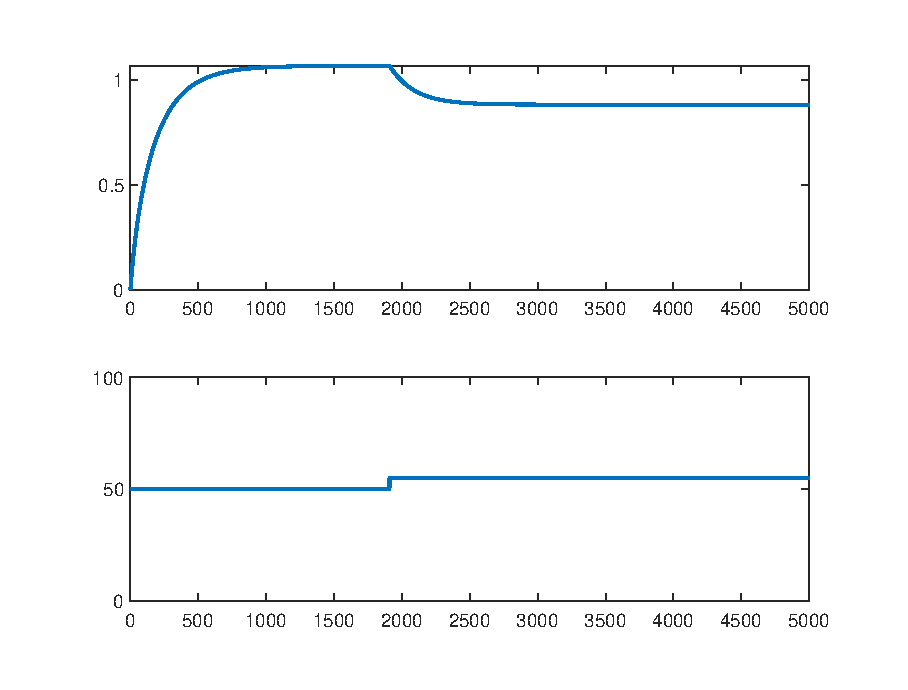
\includegraphics[scale=0.9]{Imagens/1_2.eps}
         \caption{Em cima: Valor de h[m] em função do tempo; Em baixo: Valor de u [\%] em função do tempo}
 	\label{fig:1}     
    \end{center}   
\end{figure}

\newpage

\subsection*{P3}
\justifying{Os valores de h(0) utilizados foram:}
\begin{itemize}
    \item 0.0m
    \item 0.25m
    \item 0.5m
    \item 0.75m
    \item 1.0m
    \item 1.0662m
    \item 1.25m
    \item 1.5m
\end{itemize}
\quad \justifying{Notar que o valor 1.0662m é o valor de equilíbrio e como tal a linha horizontal tracejada que se observa na figura.}

\begin{figure} [H]
    \begin{center}
        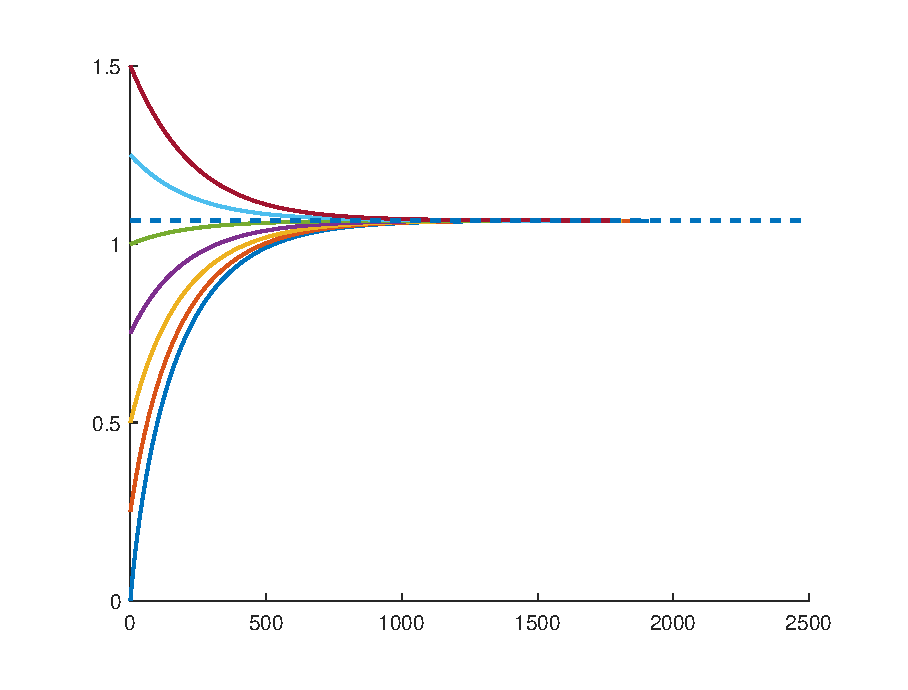
\includegraphics[width = 0.9 \textwidth]{Imagens/1_3.eps}
         \caption{Variação da altura \textit{h} em função do tempo para diferentes valores de \textit{h(0)} iniciais}
 	\label{fig:2}     
    \end{center}   
\end{figure}


\subsection*{P4}
\quad \justifying{A solução da equação \ref{difeq} é dada quando $\frac{dh}{dt}=0$. O que resulta na equação:}
\begin{equation}
    h_0=\left( \frac{10^{-3}Q}{ub\sqrt{2g}}\right)^2   
\end{equation}\\
\quad \quad \justifying{Daqui observamos que o ponto de equilíbrio é inversamente proporcional a $u^2$ o que é corroborado pelos dados da figura \ref{fig:1} onde quando \textit{u} sobe para 55\% o ponto de equilíbrio desce. Podemos também concluir que o ponto de equilíbrio não depende das condições iniciais e olhando para a equação \ref{difeq}, quando o valor de \textit{h} é $h_0^+$ vemos que o valor da derivada é negativo e quando é $h_0^-$ é positivo. Ambas estas propriedades podem ser observadas na figura \ref{fig:2}.

\end{document}

